\lecture{Лекция 8}{lec8}
\subtitle{Лекция 8 --- Алгоритмы и исполнители}

\frame[plain]
{\titlepage}	% Титульный слайд


\begin{frame}
\frametitle{Алгоритмы и исполнители}

\begin{center}

\Huge
Понятие и свойства алгоритма
	
\end{center}
\end{frame}

	\begin{frame}
\frametitle{Интуитивное понятие алгоритма}

Происхождение самого слова <<алгоритм>> связано с именем арабского ученого Мухаммеда ал-Хорезми, жившего в IX веке в Багдаде при дворе халифа ал-Мамуна.\\ На основании его трудов в средние века были сформулированы основные правила арифметики, которыми мы пользуемся до сих пор. 

В латинском переводе все правила начинались со слов <<ал-Хорезми сказал>>, что потом трансформировалось в 
<<алгоритм гласит>>.

\end{frame}

\begin{frame}
\frametitle{Интуитивное понятие алгоритма}

В течение столетий этот термин приобретал все более широкое значение и все глубже входил в науку. Сегодня слово <<алгоритм>> используют как для обозначения некоторого процесса, так и для его информационной модели – описания этого процесса. 

Поскольку никакой путаницы при этом, как правило, не возникает, то мы тоже будем считать понятия <<алгоритм>> и <<алгоритмический процесс>> синонимичными.

\end{frame}

\begin{frame}
\frametitle{Интуитивное понятие алгоритма}

\begin{exampleblock}{Определение}
Алгоритм – точное и понятное пpедписание исполнителю совеpшить последовательность действий, направленных на решение поставленной задачи.

\end{exampleblock}

Алгоритм --- одно из основных понятий информатики и математики.
\end{frame}

\subsection{Свойства алгоpитма}
	\begin{frame}
\frametitle{Свойства алгоpитма}

В соответствии с интуитивным понятием алгоритма некий процесс может быть назван алгоритмическим, если он отвечает следующим требованиям:
\begin{itemize}

\item дискретность;

\item детерминированность;

\item результативность;

\item массовость.
\end{itemize}
\end{frame}

\begin{frame}
\frametitle{Свойства алгоpитма}
\begin{block}{Дискретность}
 Дискретность означает возможность разделения процесса на взаимозависимые последовательные, достаточно элементарные шаги.
\end{block}



\end{frame}

\begin{frame}
\frametitle{Свойства алгоpитма}

\begin{block}{Детерминированность}
a)      процесс может быть без искажений передан от одного носителя информации к другому (в частности от одного человека к другому);\\
b)      результаты, получаемые на любой неначальной стадии процесса, полностью определяются результатами предыдущих стадий;\\
c)      каждая стадия процесса, в свою очередь, является детерминированным процессом.
\end{block}

\end{frame}

\begin{frame}
\frametitle{Свойства алгоpитма}

\begin{block}{Результативность}
Результативность означает, что применение процесса к своему классу задач дает решение через конечное число шагов.
\end{block}

\end{frame}

\begin{frame}
\frametitle{Свойства алгоpитма}

\begin{block}{Массовость}
Массовость означает возможность применения процесса к достаточно широкому классу задач.
\end{block}

\end{frame}

\subtitle{Понятие исполнителя}
\begin{frame}
\frametitle{Понятие исполнителя}

\begin{block}{Исполнитель алгоритма}
Исполнитель алгоритма --- это некоторая абстрактная или реальная (техническая, биологическая или биотехническая) система, способная выполнить действия, предписываемые алгоритмом.
\end{block}

\end{frame}

\begin{frame}
\frametitle{Понятие исполнителя}

Исполнителя хаpактеpизуют:
\begin{itemize}
\item сpеда;

\item элементаpные действия;

\item cистема команд;

\item отказы.
\end{itemize}
\end{frame}

\begin{frame}
\frametitle{Сpеда}

Сpеда (или обстановка) --- это <<место обитания>> исполнителя. 

Напpимеp, для исполнителя Pобота из школьного учебника сpеда --- это бесконечное клеточное поле. Стены и закpашенные клетки тоже часть сpеды. А их pасположение и положение самого Pобота задают конкpетное состояние среды.

\end{frame}

\begin{frame}
\frametitle{Система команд}

 Каждый исполнитель может выполнять команды только из некотоpого стpого заданного списка --- \alert{системы команд исполнителя.} 

Для каждой команды должны быть заданы условия пpименимости (в каких состояниях сpеды может быть выполнена команда) и описаны pезультаты выполнения команды. 

Напpимеp, команда Pобота <<ввеpх>> может быть выполнена, если выше Pобота нет стены. Ее pезультат --- смещение Pобота на одну клетку ввеpх.

\end{frame}

\begin{frame}
\frametitle{Элементаpное действие}

После вызова команды исполнитель совеpшает соответствующее элементаpное действие.

\end{frame}

\begin{frame}
\frametitle{Отказы}

Отказы исполнителя возникают, если команда вызывается пpи недопустимом для нее состоянии сpеды.

\end{frame}

\begin{frame}
\frametitle{Универсальный исполнитель}

Обычно исполнитель ничего не знает о цели алгоpитма. Он выполняет все полученные команды, не задавая вопросов <<почему>> и <<зачем>>.

В информатике универсальным исполнителем алгоритмов является компьютер.
\end{frame}


\begin{frame}
\frametitle{Алгоритмы и исполнители}

\begin{center}

\Huge
Примеры исполнителей	
\end{center}
\end{frame}

\begin{frame}[fragile]
\frametitle{Чертежник}
Исполнитель Чертежник перемещается на координатной плоскости, оставляя след в виде линии. Чертёжник может выполнять команду сместиться на (a, b), где a, b - целые числа. Эта команда перемещает Чертежника из точки с координатами (x, y) в точку с координатами (x + a; y + b). 
\begin{verbatim}
Цикл
ПОВТОРИ число РАЗ
  последовательность команд
КОНЕЦ ПОВТОРИ
\end{verbatim}
означает, что последовательность команд будет выполнена указанное число раз (число должно быть натуральным). 

\end{frame}

\begin{frame}[fragile]
\frametitle{Чертежник}
Чертёжнику был дан для исполнения алгоритм. Укажите наименьшее возможное значение числа n (n > 1), для которого найдутся такие значения чисел a и b, что после выполнения программы Чертёжник возвратится в исходную точку.
\begin{verbatim}
НАЧАЛО
сместиться на (–3, –3)
ПОВТОРИ n РАЗ
  сместиться на (a, b)
  сместиться на (27, 12)
КОНЕЦ ПОВТОРИ
сместиться на (–22, -7)
КОНЕЦ
\end{verbatim}
\pause Ответ 5
 


\end{frame}


\begin{frame}[fragile]
\frametitle{Робот}
Среда исполнителя --- клетчатое поле, между соседними клетками которого могут стоять стены.
Исполнитель может двигаться по полю, выполняя команду \texttt{делать <направление>}, аргументом которой  является: вверх, вниз, влево, вправо.

Каждая команда движения вызывает перемещение исполнителя на одну клетку в заданном направлении.

Если при движении на пути Робота встречается стена, то Робот разрушается (бдыщь!) и выполнение программы прекращается.


\end{frame}

\begin{frame}[fragile]
\frametitle{Робот}
Робот может определять наличие стен между клетками, выполняя проверку
\texttt{<направление> свободно}
Результатом проверки является значение ИСТИНА, если между клеткой, в которой находится исполнитель, и соседней в указанном направлении нет стены. Иначе результат ЛОЖЬ.
\begin{verbatim}
Пример:
ПОКА справа свободно
	ДЕЛАТЬ вправо
\end{verbatim}
Робот будет двигаться вправо и остановится, когда дойдет до стены.


\end{frame}

\begin{frame}[fragile]
\frametitle{Задача}
Сколько клеток данного лабиринта соответству-ют требованию, что, выполнив предложенную программу, Робот остановится в той же клетке, с которой он начал движение? В ответе запишите число – количество таких клеток.
\setlength{\columnsep}{2cm}
\begin{multicols}{2}
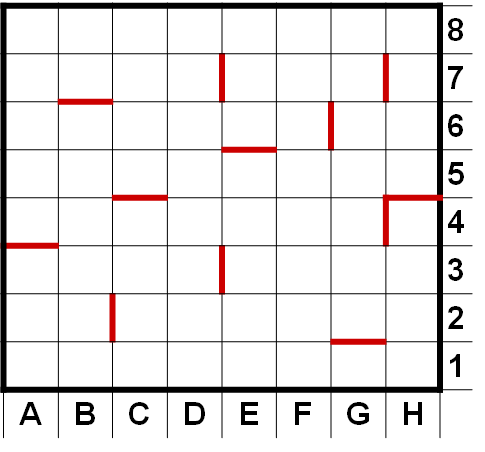
\includegraphics[height=5cm]{images/it_10}

\columnbreak
\footnotesize
\begin{verbatim}
НАЧАЛО
  ПОКА слева свободно
    ДЕЛАТЬ влево
  ПОКА сверху свободно
    ДЕЛАТЬ вверх
  ПОКА справа свободно
    ДЕЛАТЬ вправо
  ПОКА снизу свободно
    ДЕЛАТЬ вниз
КОНЕЦ
\end{verbatim}
\pause Ответ 3
\end{multicols}
\normalsize
\end{frame}

\begin{frame}[fragile]
\frametitle{Калькулятор}
Задача. У исполнителя Калькулятор две команды, которым присвоены номера:
\begin{verbatim}
1) прибавь 1,  
2) умножь на 3. 
\end{verbatim} 
Первая из них увеличивает число на 1, вторая – утраивает его. Программа для Калькулятора — это последовательность команд. Сколько существует программ, которые число 1 преобразуют в 29? 


\end{frame}

\begin{frame}[fragile]
\frametitle{Калькулятор}
\begin{enumerate}
	\item Формула количества команд $K_n=K_{n-1}+K_{\frac{n}{3}}$
	\item Составляем таблицу\\
	\begin{tabular}{c|c|c|c|c|c|c|c|c|c|c|}
\multicolumn{1}{c}{} & \multicolumn{1}{c}{0} & \multicolumn{1}{c}{1} & \multicolumn{1}{c}{2} & \multicolumn{1}{c}{3} & \multicolumn{1}{c}{4} & \multicolumn{1}{c}{5} & \multicolumn{1}{c}{6} & \multicolumn{1}{c}{7} & \multicolumn{1}{c}{8} & \multicolumn{1}{c}{9}\tabularnewline
\cline{2-11} \cline{3-11} \cline{4-11} \cline{5-11} \cline{6-11} \cline{7-11} \cline{8-11} \cline{9-11} \cline{10-11} \cline{11-11} 
0 & X & 1 & 1 & 2 & 2 & 2 & 3 & 3 & 3 & 5\tabularnewline
\cline{2-11} \cline{3-11} \cline{4-11} \cline{5-11} \cline{6-11} \cline{7-11} \cline{8-11} \cline{9-11} \cline{10-11} \cline{11-11} 
1 & 5 & 5 & 7 & 7 & 7 & 9 & 9 & 9 & 12 & 12\tabularnewline
\cline{2-11} \cline{3-11} \cline{4-11} \cline{5-11} \cline{6-11} \cline{7-11} \cline{8-11} \cline{9-11} \cline{10-11} \cline{11-11} 
2 & 12 & 15 & 15 & 15 & 18 & 18 & 18 & 23 & 23 & 23\tabularnewline
\cline{2-11} \cline{3-11} \cline{4-11} \cline{5-11} \cline{6-11} \cline{7-11} \cline{8-11} \cline{9-11} \cline{10-11} \cline{11-11} 
\end{tabular}
\end{enumerate}


\end{frame}

\begin{frame}[fragile]
\frametitle{Калькулятор}
Исполнитель Май18 преобразует число на экране. У исполнителя есть две команды, которым присвоены номера:
\begin{verbatim}
1. Прибавить 1
2. Прибавить 3
\end{verbatim} 
Сколько существует программ, для которых при исходном числе 2 результатом является число 20 и при этом траектория вычислений содержит число 10 и не содержит число 15?


\end{frame}

\begin{frame}[fragile]
\frametitle{Калькулятор}
\begin{enumerate}
	\item Формула количества команд $K_n=K_{n-1}+K_{n-3}$
	\item Составляем таблицу\\
\begin{tabular}{c|c|c|c|c|c|c|c|c|c|c|}
\multicolumn{1}{c}{} & \multicolumn{1}{c}{0} & \multicolumn{1}{c}{1} & \multicolumn{1}{c}{2} & \multicolumn{1}{c}{3} & \multicolumn{1}{c}{4} & \multicolumn{1}{c}{5} & \multicolumn{1}{c}{6} & \multicolumn{1}{c}{7} & \multicolumn{1}{c}{8} & \multicolumn{1}{c}{9}\tabularnewline
\cline{2-11} \cline{3-11} \cline{4-11} \cline{5-11} \cline{6-11} \cline{7-11} \cline{8-11} \cline{9-11} \cline{10-11} \cline{11-11} 
0 & X & X & 1 & 1 & 1 & 2 & 3 & 4 & 6 & 9\tabularnewline
\cline{2-11} \cline{3-11} \cline{4-11} \cline{5-11} \cline{6-11} \cline{7-11} \cline{8-11} \cline{9-11} \cline{10-11} \cline{11-11} 
1 & 13 & 13 & 13 & 26 & 39 & X & 26 & 65 & 65 & 91\tabularnewline
\cline{2-11} \cline{3-11} \cline{4-11} \cline{5-11} \cline{6-11} \cline{7-11} \cline{8-11} \cline{9-11} \cline{10-11} \cline{11-11} 
2 & 156 & X & X & X & X & X & X & X & X & X\tabularnewline
\cline{2-11} \cline{3-11} \cline{4-11} \cline{5-11} \cline{6-11} \cline{7-11} \cline{8-11} \cline{9-11} \cline{10-11} \cline{11-11} 
\end{tabular}
\end{enumerate}


\end{frame}

\begin{frame}[fragile]
\frametitle{Автомат}
Задача. Автомат получает на вход четырёхзначное число. По этому числу строится новое число по следующим правилам:
1. Складываются первая и вторая, а также третья и четвёртая цифры исходного числа.\\
2. Полученные два числа записываются друг за другом в порядке убывания (без разделителей).

Пример. Исходное число: 3165. Суммы: 3 + 1 = 4; 6 + 5 = 11. Результат: 114.

Укажите наименьшее число, в результате обработки которого, автомат выдаст число 1311.

\pause Ответ:  2949.
\end{frame}

\begin{frame}[fragile]
\frametitle{Редактор}
Задача. Редактор получает на вход строку цифр и преоб-разовывает её. Редактор может выполнять две команды, в обеих командах v и w обозначают цепочки цифр.\\
\texttt{А) заменить (v, w)}\\
Эта команда заменяет в строке первое слева вхождение цепочки v на цепочку w. \\
\texttt{Б) нашлось (v)}\\
Эта команда проверяет, встречается ли цепочка v в строке исполнителя Редактор. Если она встречается, то команда возвращает логическое значение «истина», в противном случае возвращает значение «ложь». Строка при этом не изменяется.

\end{frame}

\begin{frame}[fragile]
\frametitle{Редактор}
Дана программа для исполнителя Редактор. Какая строка получится в результате применения приведённой выше программы к строке, состоящей из 68 идущих подряд цифр 8? В ответе запишите полученную строку. 
\small
\begin{verbatim}
НАЧАЛО
 ПОКА нашлось (222) ИЛИ нашлось (888)
  ЕСЛИ нашлось (222)
			ТО заменить (222, 8)
	ИНАЧЕ заменить (888, 2)
	КОНЕЦ ЕСЛИ
 КОНЕЦ ПОКА
КОНЕЦ
\end{verbatim}
\normalsize
\pause Ответ:  28.
\end{frame}